%% Springer Nature LaTeX template — npj Microgravity style.
%% Class file (sn-jnl.cls) + bib style (sn-nature.bst) are provided by the
%% official Springer Nature template. Easiest route: open this folder on
%% Overleaf using the "Springer Nature Article Template" (see README.md).
\documentclass[pdflatex,sn-nature]{sn-jnl}

\usepackage{graphicx}
\usepackage{multirow}
\usepackage{amsmath,amssymb,amsfonts}
\usepackage{booktabs}
\usepackage{textcomp}
\usepackage{xcolor}

\graphicspath{{figures/}}

\begin{document}

\title[Conserved mitochondrial suppression across six species]{Conserved
mitochondrial suppression and organelle-specific transcriptomic responses to
spaceflight across six eukaryotic species}

%% TODO: confirm author list, ORCID, and affiliation before submission.
\author[1]{\fnm{Richard} \sur{Barker}}
\affil[1]{\orgname{The Collaborative Science Environment},
  \email{admin@cosecloud.com}}

\abstract{Spaceflight induces transcriptomic changes across organisms, but the
extent to which subcellular and metabolic pathways are conserved across species
remains poorly understood. We performed a cross-species meta-analysis of 22
transcriptomic datasets from the NASA Open Science Data Repository spanning six
eukaryotic species (\textit{Homo sapiens}, \textit{Mus musculus},
\textit{Drosophila melanogaster}, \textit{Caenorhabditis elegans},
\textit{Saccharomyces cerevisiae}, and \textit{Arabidopsis thaliana}),
encompassing 20{,}333 differentially expressed genes (DEGs). Using a
human-anchored orthology matrix built from OrthoDB v12 (18{,}030 genes, 651 with
orthologs in all five other species), we mapped DEGs to 16 subcellular
compartments and applied Fisher's combined probability test to identify conserved
organelle-level responses. We report a striking conserved downregulation of
mitochondrial genes: 49 orthologs show significant, direction-consistent
suppression across at least three species (Fisher FDR \(< 0.05\), minimum \(p =
7.7 \times 10^{-68}\)), including components of Complex III (CYC1), Complex IV
(COX5B, COX6A2, COX6B2), ATP synthase (ATP5F1A, ATP5PD), and the TCA cycle
(IDH3A, IDH3B, IDH3G). In contrast, peroxisome, lipid droplet, and Golgi
apparatus genes show conserved upregulation. KEGG pathway visualization with
per-species log2FC overlays reveals that NAD\textsuperscript{+}-dependent
oxidative phosphorylation enzymes are divergently regulated (down in fly, up in
human and mouse), while CoA-dependent TCA cycle enzymes are broadly conserved.
These findings identify mitochondrial energy metabolism as a deeply conserved
target of the spaceflight transcriptional response across a billion years of
eukaryotic evolution.}

\keywords{spaceflight, transcriptomics, mitochondria, cross-species meta-analysis,
NASA OSDR, orthology}

\maketitle

\section{Introduction}\label{sec:intro}

Spaceflight exposes organisms to a unique combination of environmental stressors
including microgravity, cosmic radiation, altered atmospheric composition, and
circadian disruption. These conditions induce measurable transcriptomic changes
across diverse organisms, from yeast to humans \cite{beheshti2021cell,galazka2021}.
The NASA Open Science Data Repository (OSDR) has accumulated hundreds of
spaceflight omics datasets through the GeneLab consortium, providing an
unprecedented opportunity for cross-species comparative analysis \cite{ray2019}.

Individual species studies have identified recurrent themes in the spaceflight
transcriptomic response, including altered energy metabolism, oxidative stress,
immune dysregulation, and cytoskeletal remodeling \cite{beheshti2020,herranz2020}.
However, most analyses have been conducted within single species, making it
difficult to distinguish conserved fundamental responses from species-specific
adaptations. A rigorous cross-species comparison requires orthology-based
integration, which maps genes across species to their common ancestral
equivalents.

Subcellular localization provides a functional organizing principle for
interpreting transcriptomic changes. Gene Ontology Cellular Component (GOCC)
enrichment can identify which organelles are coordinately regulated, and
cross-species conservation of these organelle-level responses would suggest
deeply rooted cellular mechanisms. Mitochondria are of particular interest given
their central role in energy metabolism, oxidative stress response, and
apoptosis, all of which are affected by spaceflight \cite{dasilva2021,mao2021}.

Here we present a cross-species meta-analysis of 22 spaceflight transcriptomic
datasets spanning six eukaryotic species. We build a human-anchored orthology
matrix using OrthoDB v12, perform subcellular location enrichment, and apply
Fisher's combined probability test to identify conserved organelle-level
responses. We further visualize conserved metabolic pathways with per-species
expression overlays and map cofactor dependencies. Our analysis reveals that
mitochondrial gene suppression is the most robustly conserved subcellular
response to spaceflight across a billion years of eukaryotic evolution.

\section{Results}\label{sec:results}

\subsection{Dataset overview and differential expression}

We queried the NASA OSDR Biological Data API for RNA-seq and microarray datasets
with spaceflight versus ground control contrasts across six species. The final
selection comprised 22 datasets: 7 mouse, 4 human, 3 Arabidopsis, 3 fly, 4 worm
(microarray), and 1 yeast (microarray) (Fig.~\ref{fig1}A). RNA-seq datasets used
GeneLab Research Community Portal (RCP) pre-computed DESeq2 tables; microarray
datasets used limma. For two datasets without pre-computed tables (OSD-96,
OSD-35), we performed de novo differential expression analysis.

We applied tiered DEG thresholds to accommodate dataset-specific statistical
power: standard (\(p_{\mathrm{adj}} < 0.05\), \(|\text{log2FC}| > 1\)) for 19
datasets, relaxed (\(p_{\mathrm{adj}} < 0.10\), \(|\text{log2FC}| > 0.5\)) for two
low-power datasets, and nominal (\(p < 0.05\), \(|\text{log2FC}| > 0.5\)) for one
dataset without replicates. This yielded 20{,}333 DEGs total, with substantial
variation across species: Arabidopsis (9{,}930), \textit{C.\ elegans} (5{,}022),
mouse (2{,}103), fly (1{,}881), human (1{,}366), and yeast (31)
(Fig.~\ref{fig1}B). The low yeast count reflects the single microarray dataset
with a relaxed threshold. Across all species, 10{,}931 DEGs were upregulated and
9{,}402 downregulated in spaceflight relative to ground controls.

\begin{figure}[htbp]
\centering
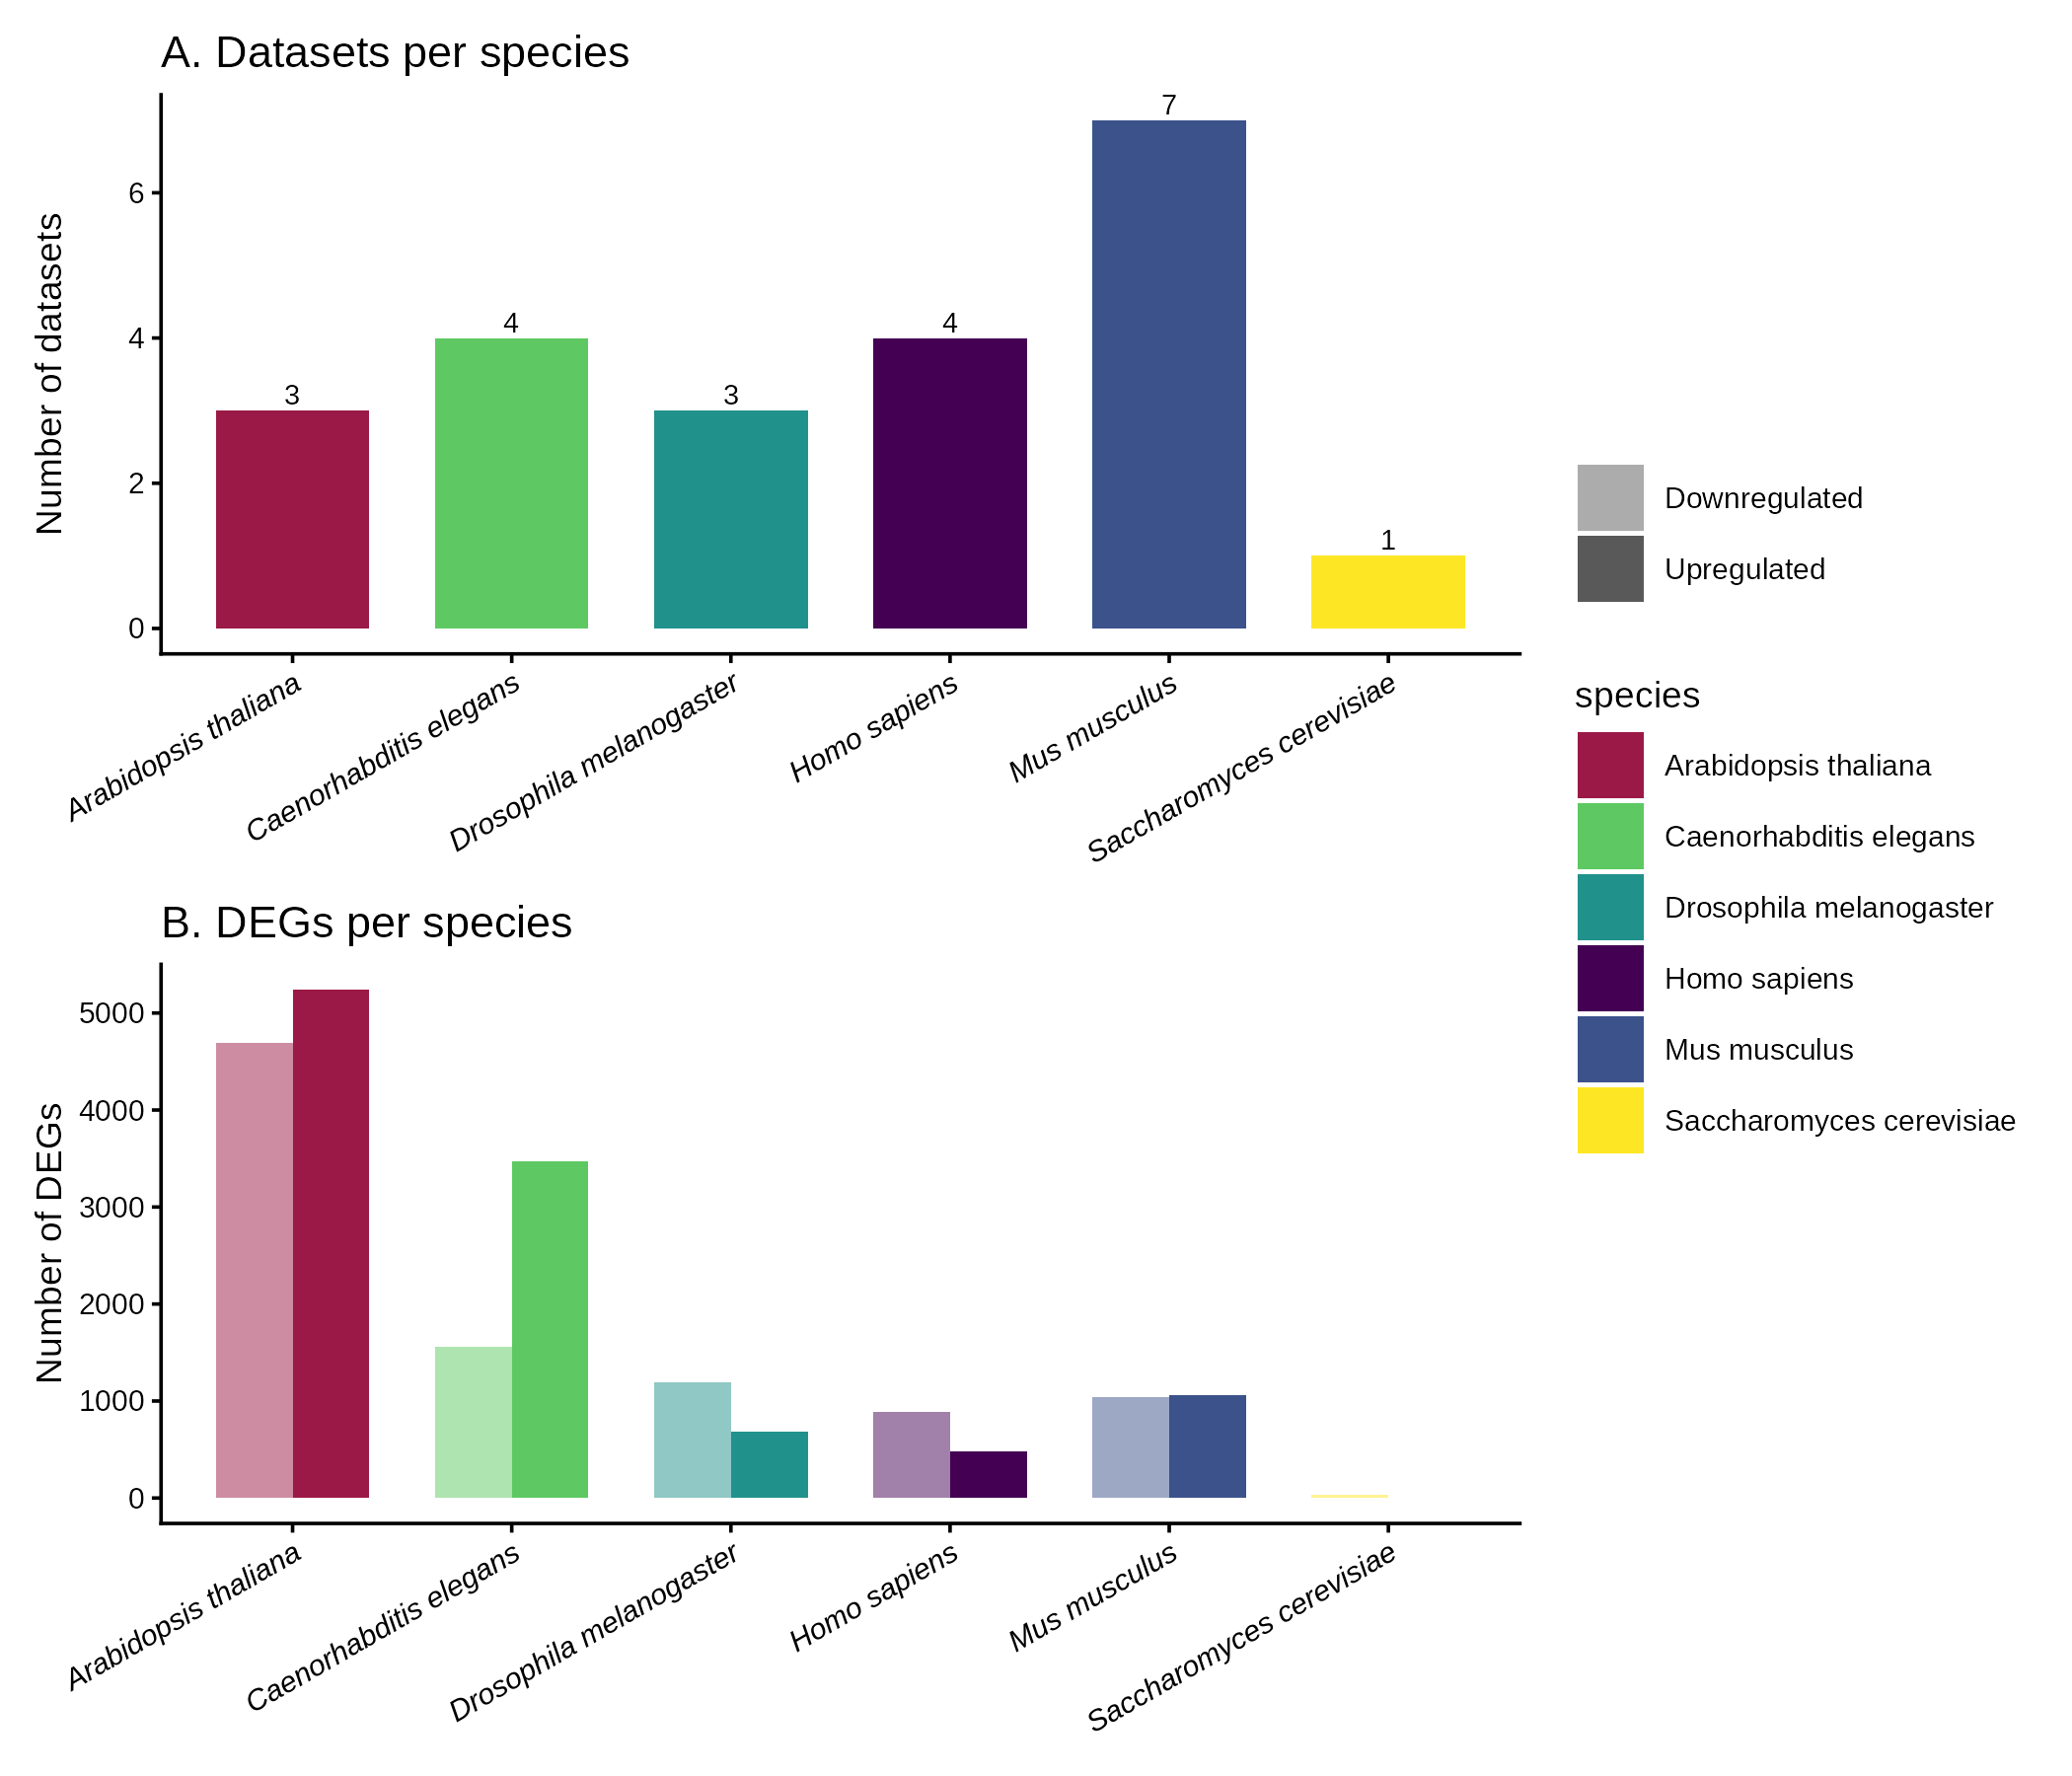
\includegraphics[width=\textwidth]{fig1_study_overview.png}
\caption{\textbf{Study overview.} (A) Number of OSDR datasets per species
included in the analysis. (B) Number of differentially expressed genes (DEGs) per
species, separated by direction (upregulated vs.\ downregulated in spaceflight
relative to ground control). Species colors are fixed globally across all figures
using a viridis-based colorblind-friendly palette.}
\label{fig1}
\end{figure}

\subsection{Human-anchored orthology mapping}

To enable cross-species comparison, we built a human-anchored orthology matrix
using OrthoDB v12 as the primary resource, supplemented by babelgene for
human-to-mouse, fly, worm, and yeast mappings. Arabidopsis orthology was mapped
via OrthoDB Eukaryota-level ortholog groups, as babelgene does not support plant
species. The unified matrix comprises 18{,}030 human genes with at least one
non-human ortholog, of which 651 have orthologs in all five other species,
3{,}446 in at least four, and 8{,}505 in at least three (Fig.~\ref{fig3}).

DEG-to-ortholog mapping rates varied substantially across species, reflecting
both evolutionary distance and gene identifier compatibility: human 100\%, mouse
70.7\%, yeast 64.5\%, fly 28.6\%, worm 18.8\%, and Arabidopsis 3.2\%. The low
Arabidopsis rate reflects the large plant-specific gene complement and the
reliance on OrthoDB rather than babelgene for plant orthology. Despite this, 352
human orthologs were identified as DEGs in two or more species, and 33 in three
or more, providing a robust foundation for conservation analysis.

\begin{figure}[htbp]
\centering
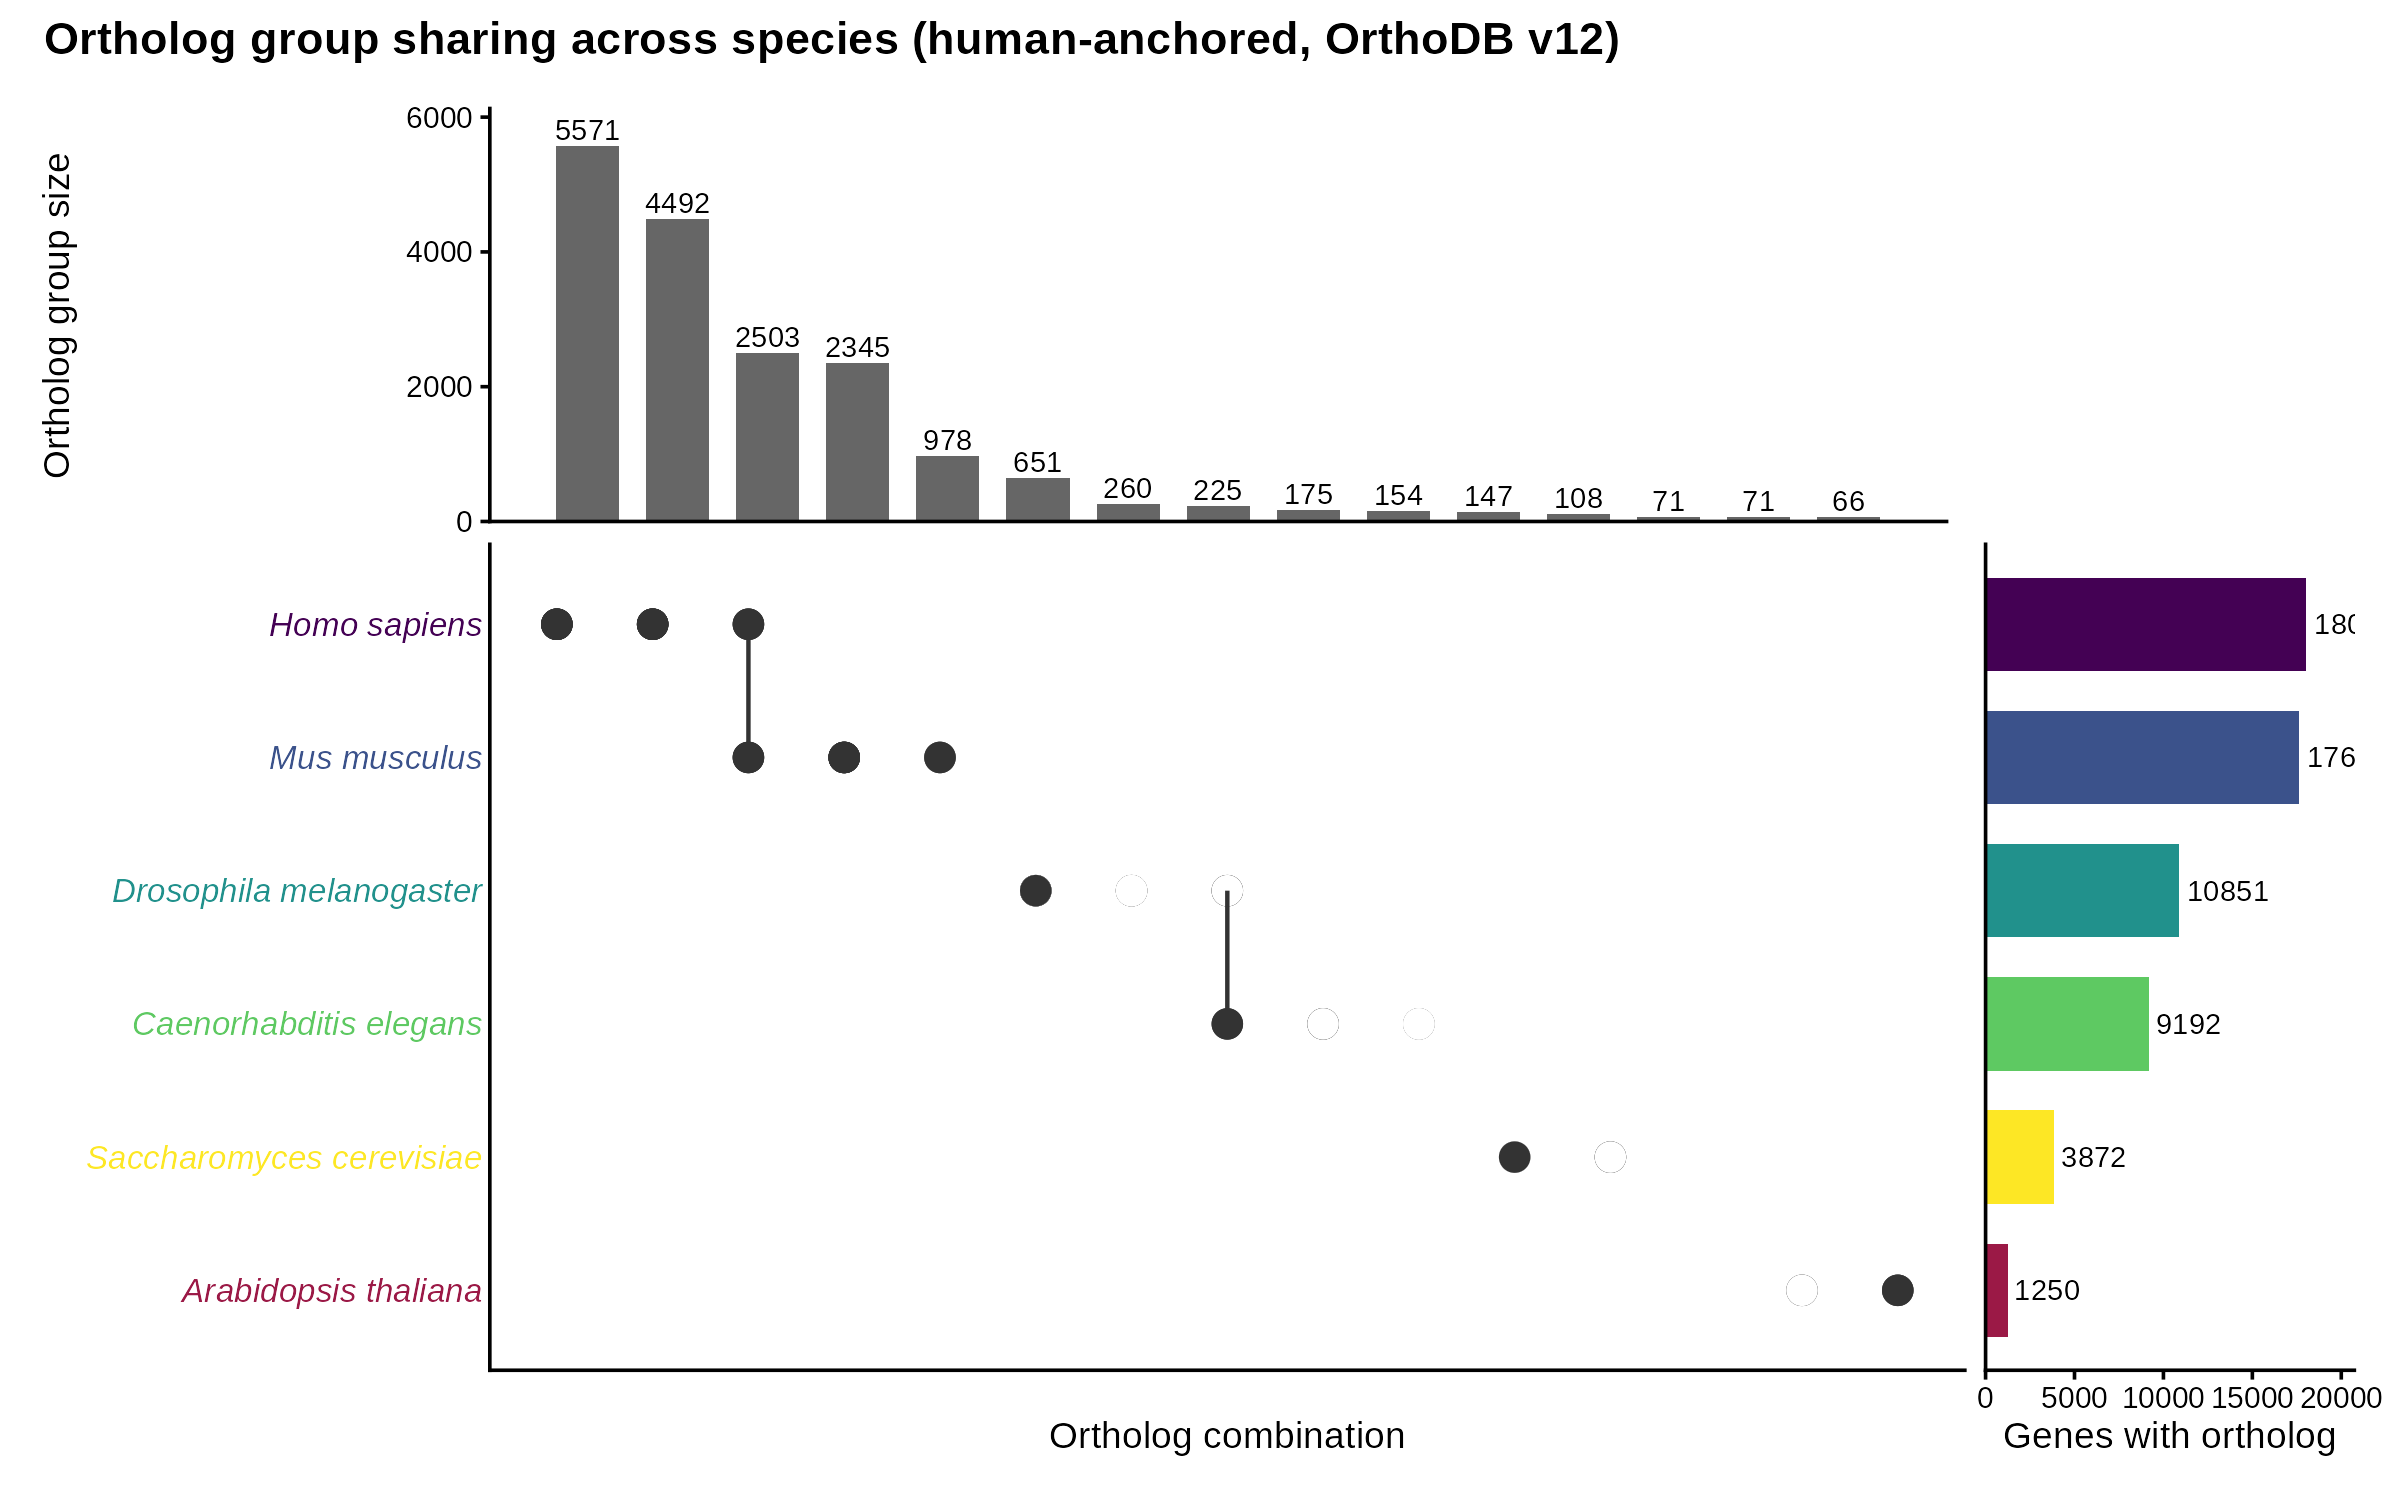
\includegraphics[width=\textwidth]{fig3_orthology_upset.png}
\caption{\textbf{Ortholog group sharing across species.} UpSet plot showing the
number of human genes with orthologs in each combination of the five non-human
species (OrthoDB v12 + babelgene). Human is the anchor species (present in all
groups). 651 genes have orthologs in all five non-human species; 8{,}505 in at
least three.}
\label{fig3}
\end{figure}

\subsection{Species-specific transcriptional responses}

Volcano plots for representative datasets (the dataset with the most DEGs per
species) reveal both shared and species-specific patterns (Fig.~\ref{fig2}). All
species show a predominance of downregulated genes in the most affected datasets,
particularly in fly (OSD-207, 1{,}735 DEGs) and human (OSD-684, 971 DEGs).
Arabidopsis (OSD-217) shows an unusually high DEG count (9{,}069), likely
reflecting the strong sensitivity of plant transcriptomes to the combined
stressors of spaceflight including altered gravity and light conditions.

\begin{figure}[htbp]
\centering
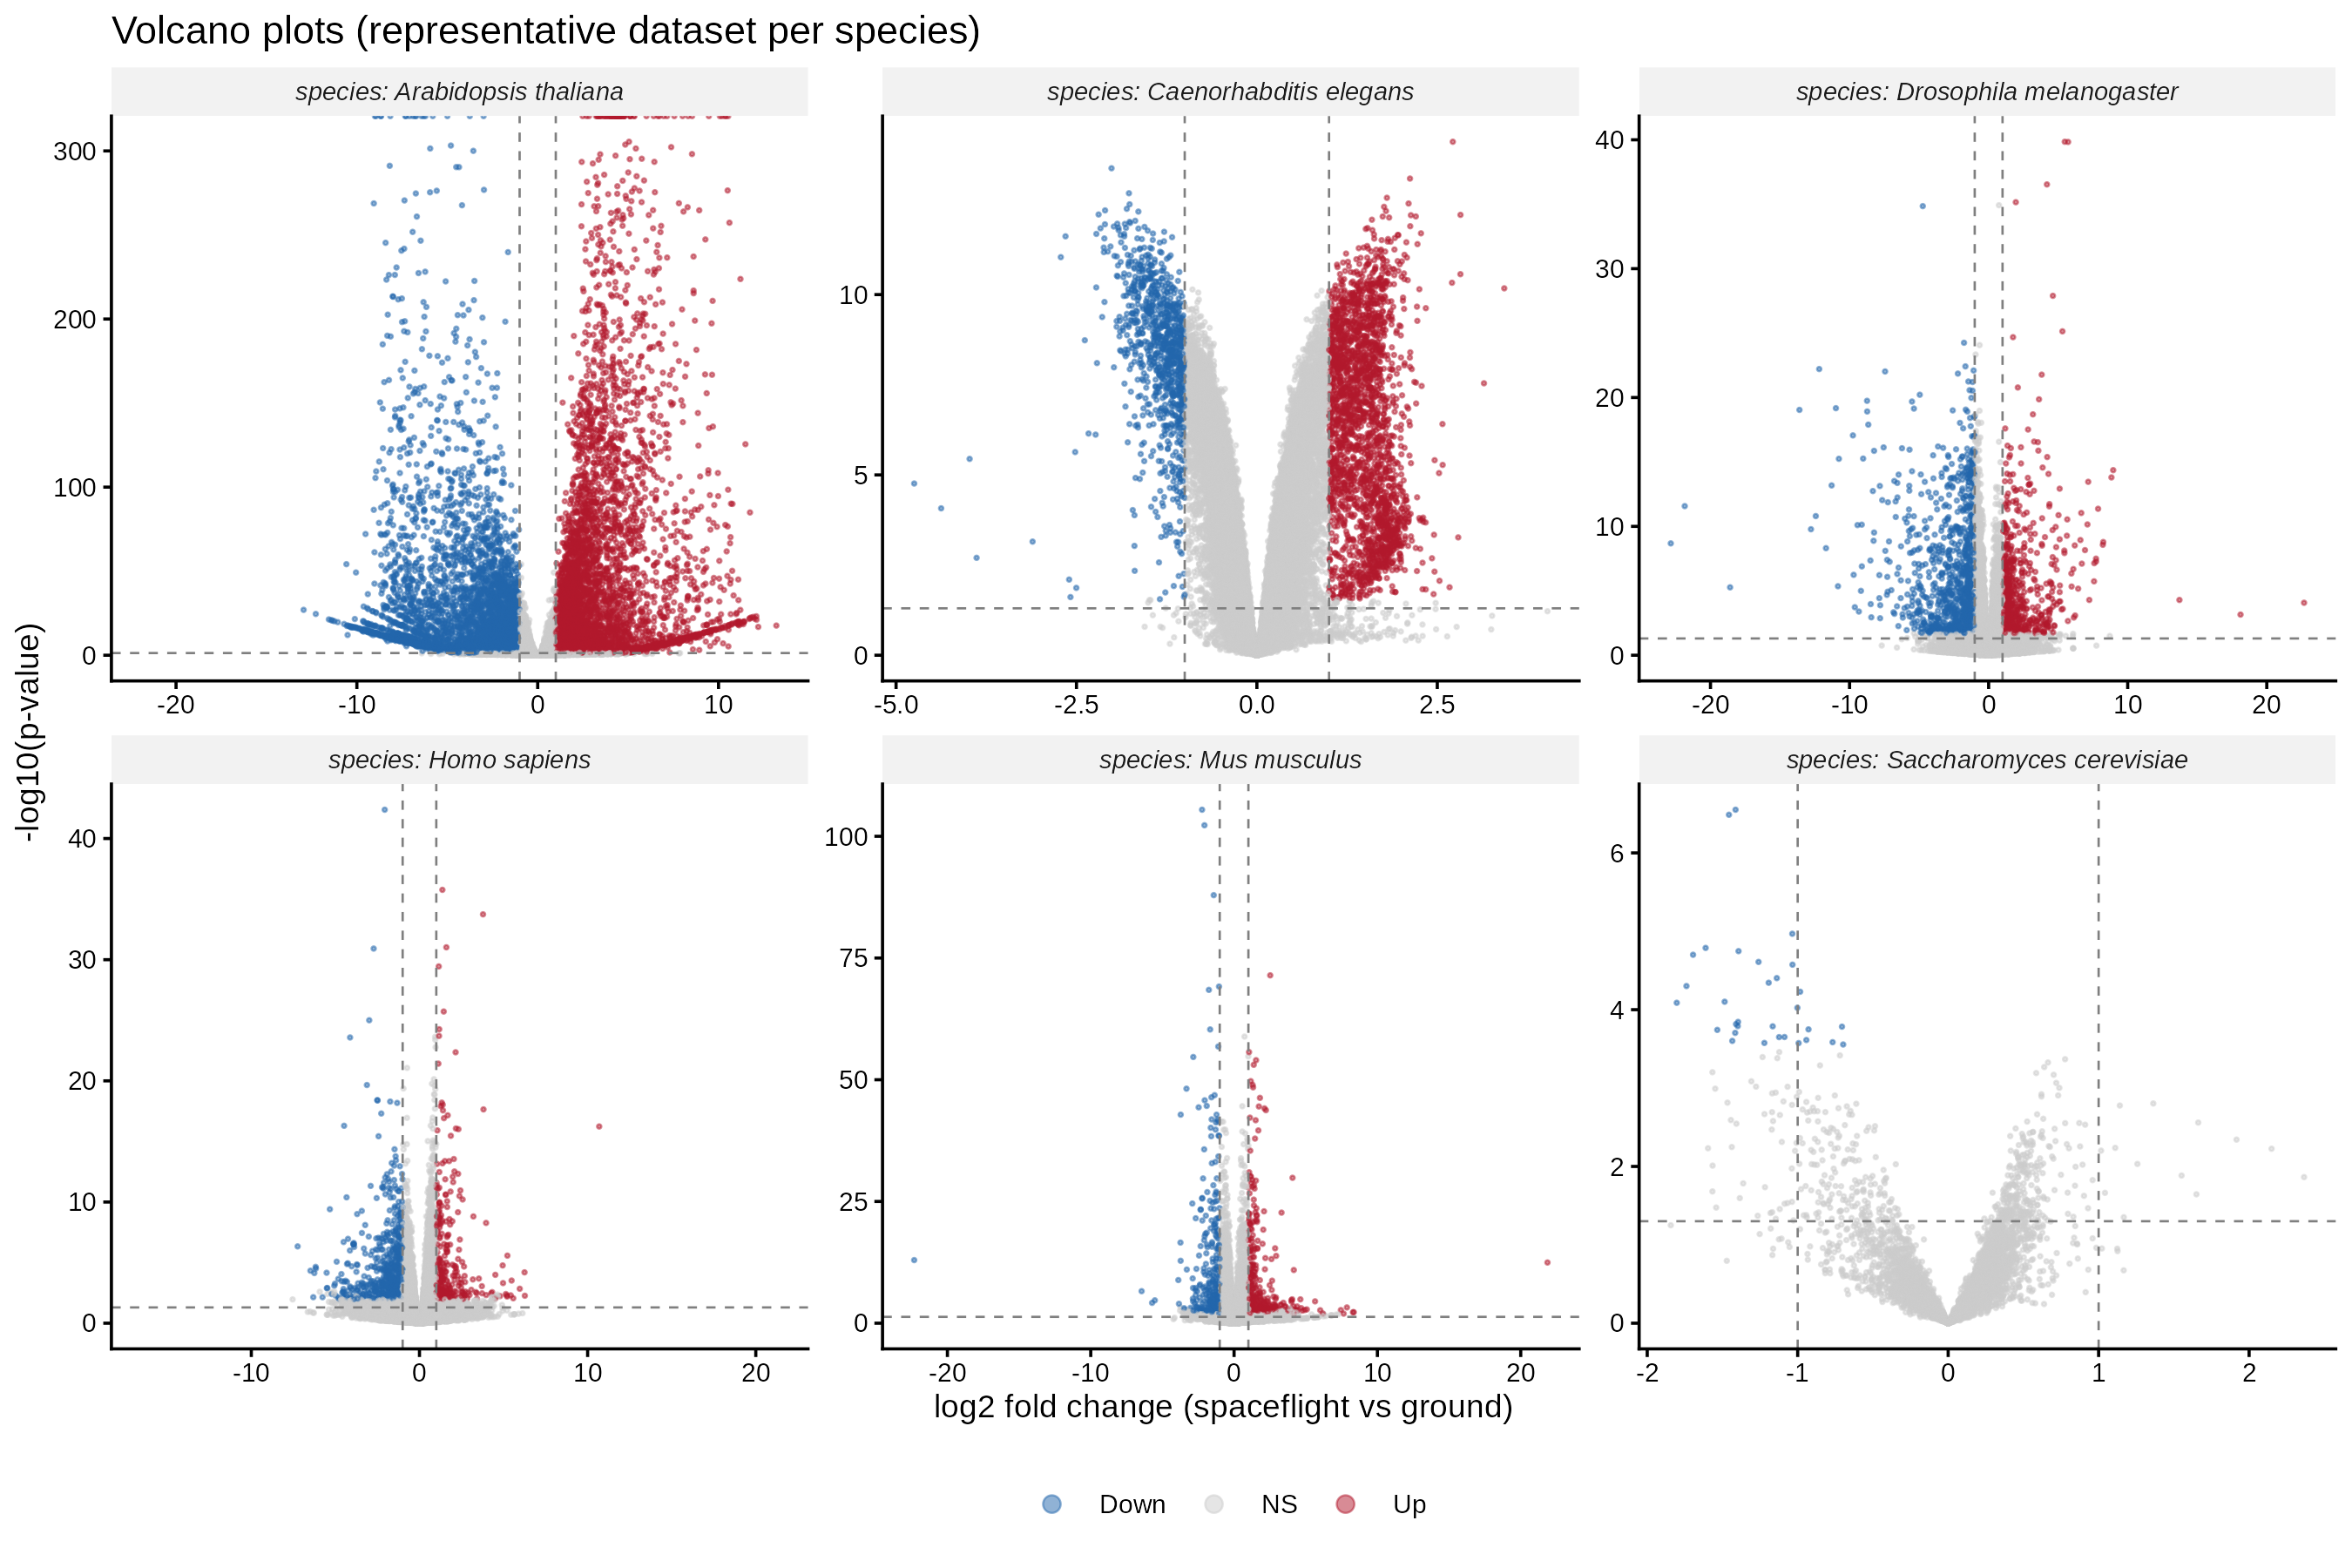
\includegraphics[width=\textwidth]{fig2_volcano_plots.png}
\caption{\textbf{Volcano plots of representative datasets per species.} Each panel
shows the dataset with the most DEGs for that species. Dashed lines indicate \(p
= 0.05\) (horizontal) and \(|\text{log2FC}| = 1\) (vertical). Red = upregulated in
spaceflight, blue = downregulated, grey = not significant. OSD IDs: Arabidopsis
OSD-217, \textit{C.\ elegans} OSD-112, Fly OSD-207, Human OSD-684, Mouse OSD-104,
Yeast OSD-62.}
\label{fig2}
\end{figure}

\subsection{Subcellular location enrichment reveals organelle-specific responses}

We performed GOCC enrichment analysis per species for up- and down-regulated DEGs
separately using clusterProfiler, yielding 200 enriched terms. We manually
classified all terms into 16 organelle categories. Seven categories were enriched
in three or more species: cell wall/extracellular matrix, plasma membrane,
extracellular, cytoskeleton, nucleus, proteasome, and ribosome (Fig.~\ref{fig4}).

The signed enrichment score (negative for downregulated, positive for
upregulated) reveals a striking pattern: mitochondrion, membrane transport,
cytoskeleton, and endoplasmic reticulum show predominantly negative scores
(downregulated enrichment) across species, while peroxisome, lipid particle,
Golgi apparatus, and chloroplast show positive scores (upregulated enrichment).
The nucleus shows a mixed response with both up- and down-regulated components,
consistent with its diverse functional roles.

\begin{figure}[htbp]
\centering
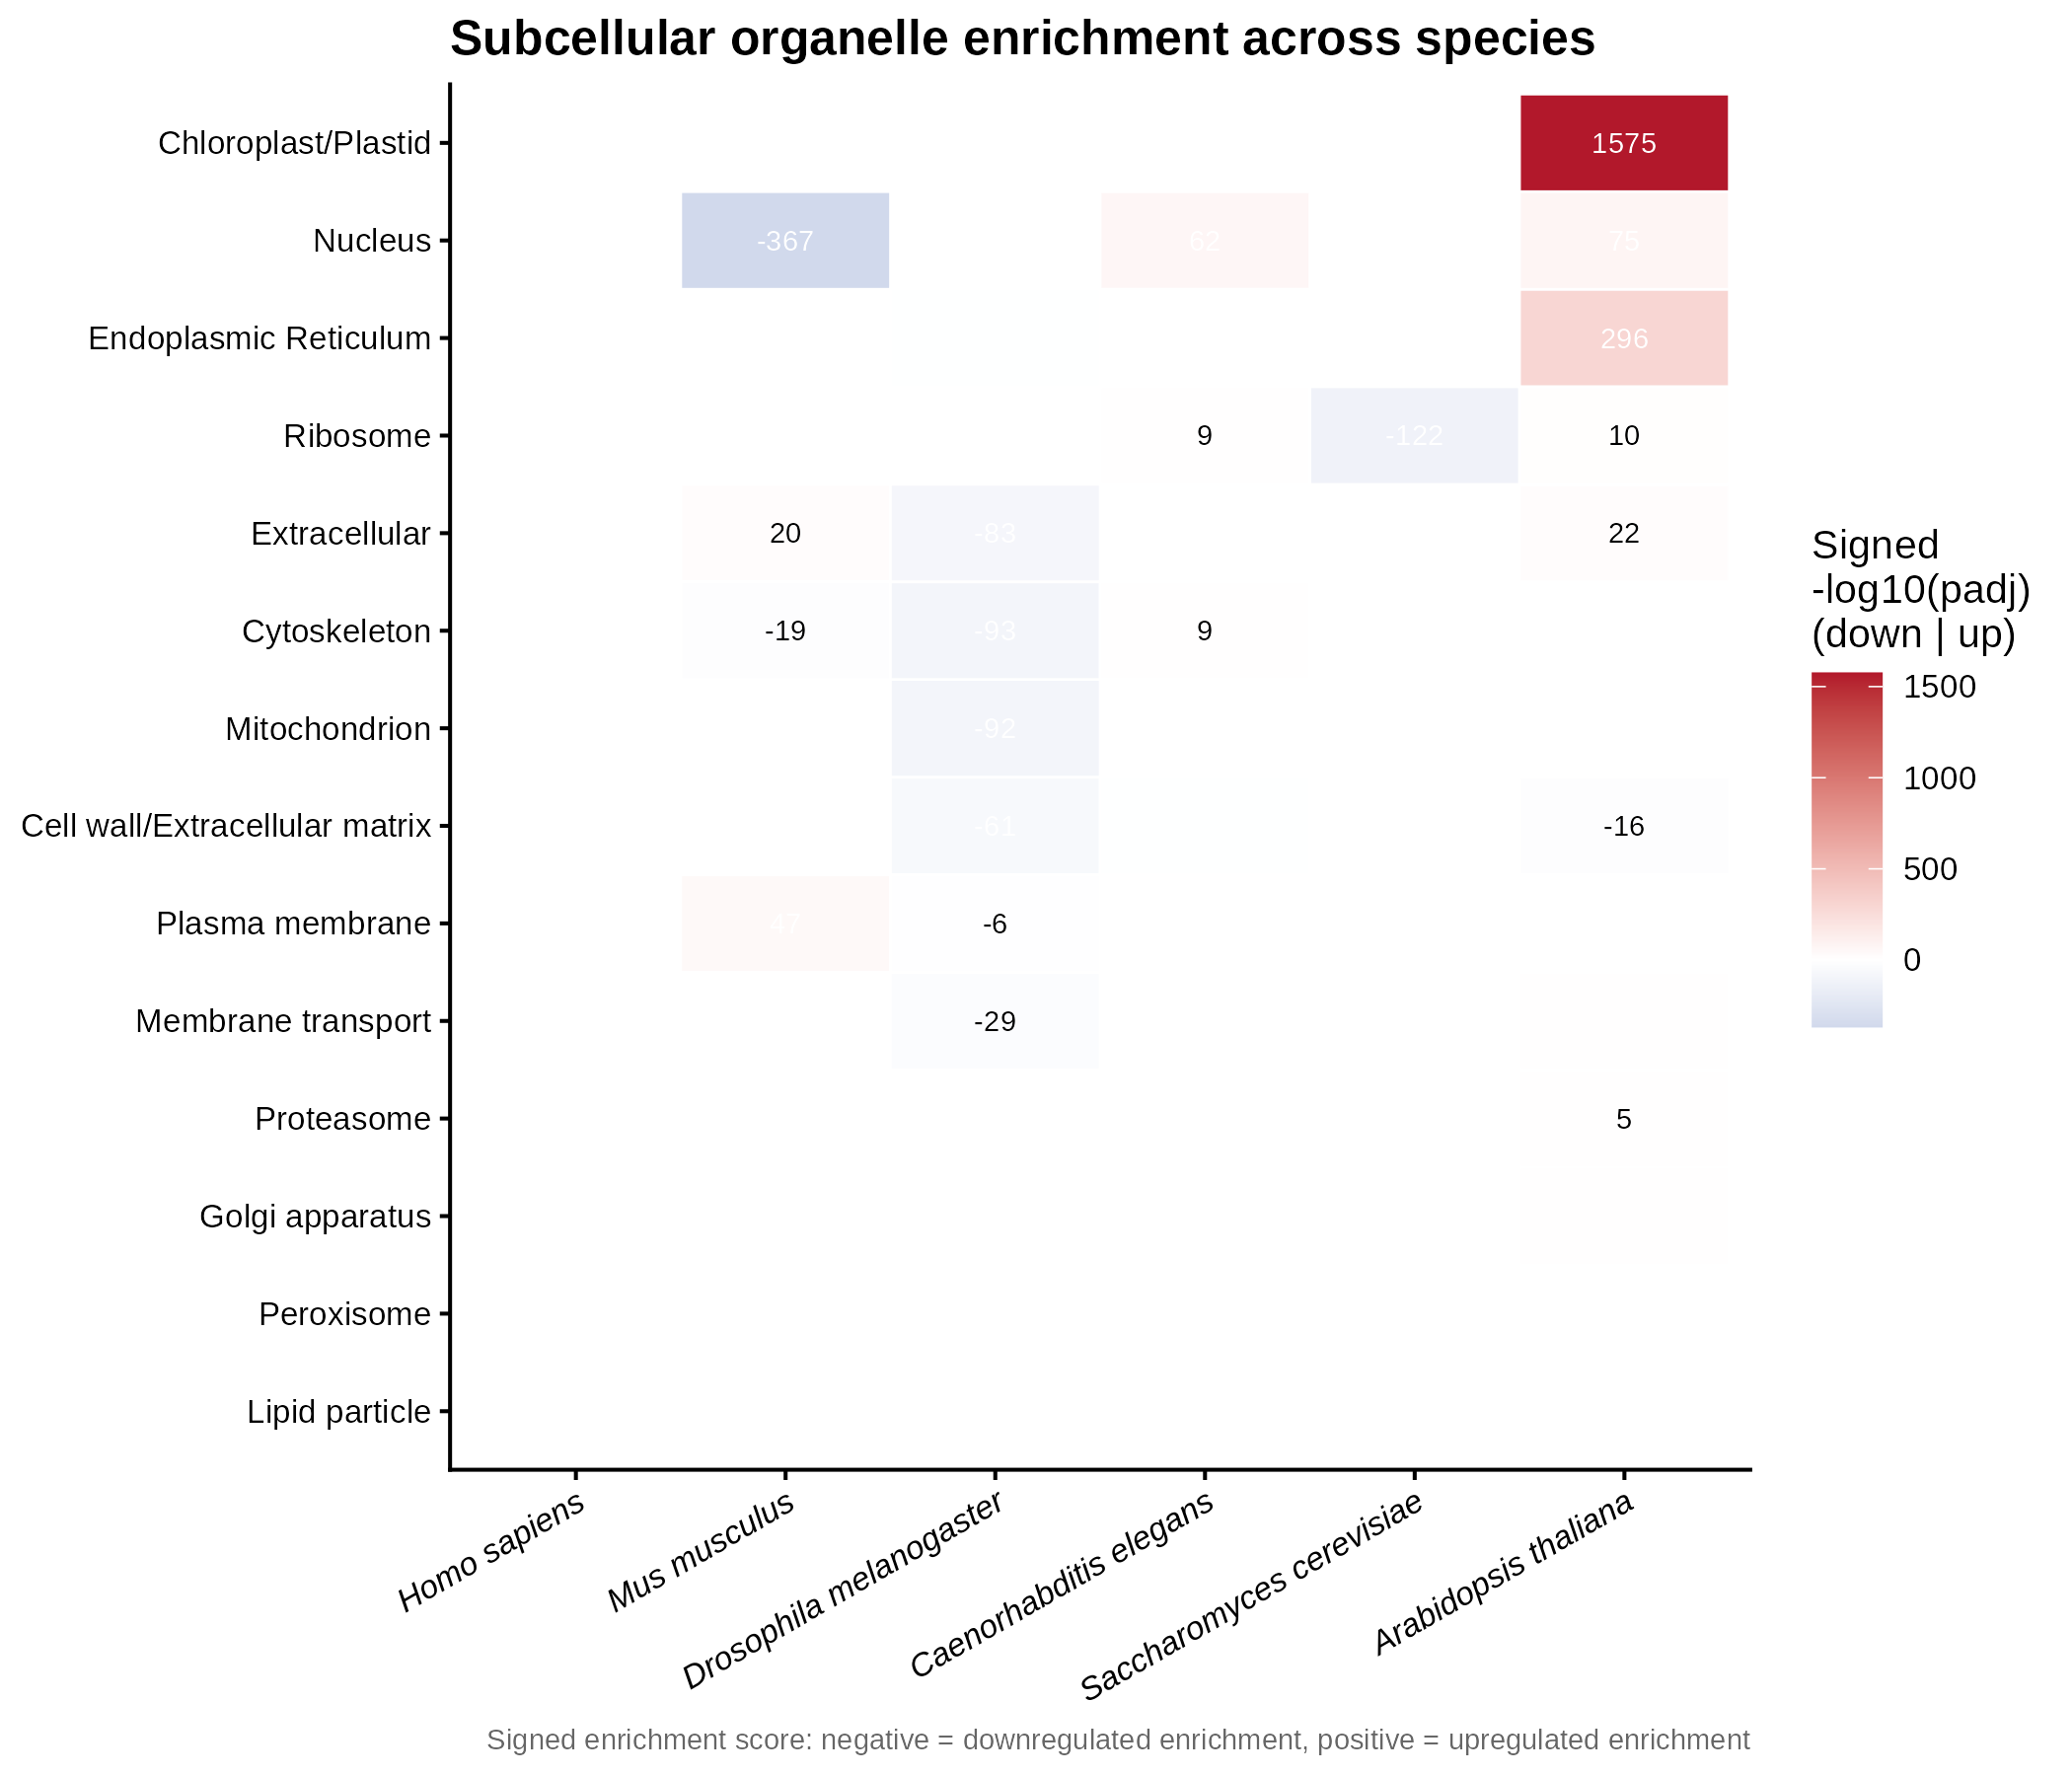
\includegraphics[width=\textwidth]{fig4_organelle_enrichment_heatmap.png}
\caption{\textbf{Subcellular organelle enrichment across species.} Heatmap shows
signed enrichment scores (sum of \(-\log_{10}\) adjusted \(p\)-value, signed by
direction) for each organelle category and species. Blue = downregulated
enrichment, red = upregulated enrichment. Organelles are ordered by total
absolute enrichment signal.}
\label{fig4}
\end{figure}

\subsection{Conserved mitochondrial suppression across species}

To formally test for cross-species conservation, we applied Fisher's combined
probability test to the per-species \(p\)-values of each orthologous gene within
each organelle category. Of 1{,}210 ortholog-organelle tests, 1{,}079 were
significant after Benjamini-Hochberg FDR correction (FDR \(< 0.05\)). We defined a
gene as `conserved' if it was significant in at least three species with
consistent direction (\(\geq 80\%\) same direction).

The most striking finding is the conserved downregulation of mitochondrial genes:
49 orthologs show significant, direction-consistent suppression across at least
three species (100\% downregulated, minimum Fisher FDR \(= 7.7 \times 10^{-68}\))
(Table~\ref{tab1}, Fig.~\ref{fig5}). The top genes include components of all major
oxidative phosphorylation complexes and the TCA cycle: IDH3B (isocitrate
dehydrogenase, 5 species, \(p = 7.7 \times 10^{-68}\)), CYC1 (cytochrome c1,
Complex III, 6 species, \(p = 3.1 \times 10^{-39}\)), COX6A2 and COX6B2 (Complex
IV, 5 species each), COX5B (Complex IV, 5 species), ATP5F1A and ATP5PD (ATP
synthase, 5 species each), and IDH3A/IDH3G (TCA cycle, 5 species each). Notably,
two genes (CYC1 and PDHB) are conserved downregulated across all six species, and
GPD2 across all six.

\begin{table}[htbp]
\centering
\caption{Top conserved downregulated mitochondrial genes across species.}
\label{tab1}
\begin{tabular}{@{}llll r@{}}
\toprule
\textbf{Symbol} & \textbf{Function} & \textbf{Complex/Pathway} & \textbf{Species (n)} & \textbf{Fisher FDR} \\
\midrule
IDH3B   & Isocitrate dehydrogenase 3B     & TCA cycle              & 5 & \(7.7\times10^{-68}\) \\
CYC1    & Cytochrome c1                   & Complex III            & 6 & \(3.1\times10^{-39}\) \\
COX6A2  & Cytochrome c oxidase subunit 6A2 & Complex IV            & 5 & \(1.8\times10^{-27}\) \\
COX6B2  & Cytochrome c oxidase subunit 6B2 & Complex IV            & 5 & \(1.8\times10^{-27}\) \\
COX5B   & Cytochrome c oxidase subunit 5B & Complex IV             & 5 & \(5.6\times10^{-27}\) \\
ATP5F1A & ATP synthase F1 alpha           & ATP synthase           & 5 & \(9.8\times10^{-25}\) \\
IDH3G   & Isocitrate dehydrogenase 3G     & TCA cycle              & 5 & \(4.8\times10^{-24}\) \\
IDH3A   & Isocitrate dehydrogenase 3A     & TCA cycle              & 5 & \(1.3\times10^{-22}\) \\
PDHB    & Pyruvate dehydrogenase E1 beta  & Pyruvate dehydrogenase & 6 & \(6.2\times10^{-20}\) \\
ATP5PD  & ATP synthase peripheral stalk   & ATP synthase           & 5 & \(1.0\times10^{-18}\) \\
GPD2    & Glycerol-3-phosphate dehydrogenase 2 & Mitochondrial shuttle & 6 & \(7.5\times10^{-18}\) \\
SLC25A6 & ADP/ATP translocase 3           & Mitochondrial transport & 4 & \(5.4\times10^{-18}\) \\
NDUFA10 & NADH dehydrogenase 1 alpha 10   & Complex I              & 4 & \(7.5\times10^{-18}\) \\
\botrule
\end{tabular}
\end{table}

In contrast to the mitochondrial suppression, several organelle categories show
conserved upregulation: peroxisome (6 genes, 100\% up, \(p = 8.4 \times
10^{-105}\)), lipid particle (5 genes, 100\% up, \(p = 1.2 \times 10^{-21}\)), and
Golgi apparatus (2 genes, 100\% up, \(p = 3.3 \times 10^{-130}\)). The proteasome
shows a mixed response (5 conserved genes: 4 down, 1 up), and the ribosome is
nearly balanced (31 conserved: 16 down, 15 up). The full conservation summary is
provided in Table~S7.

\begin{figure}[htbp]
\centering
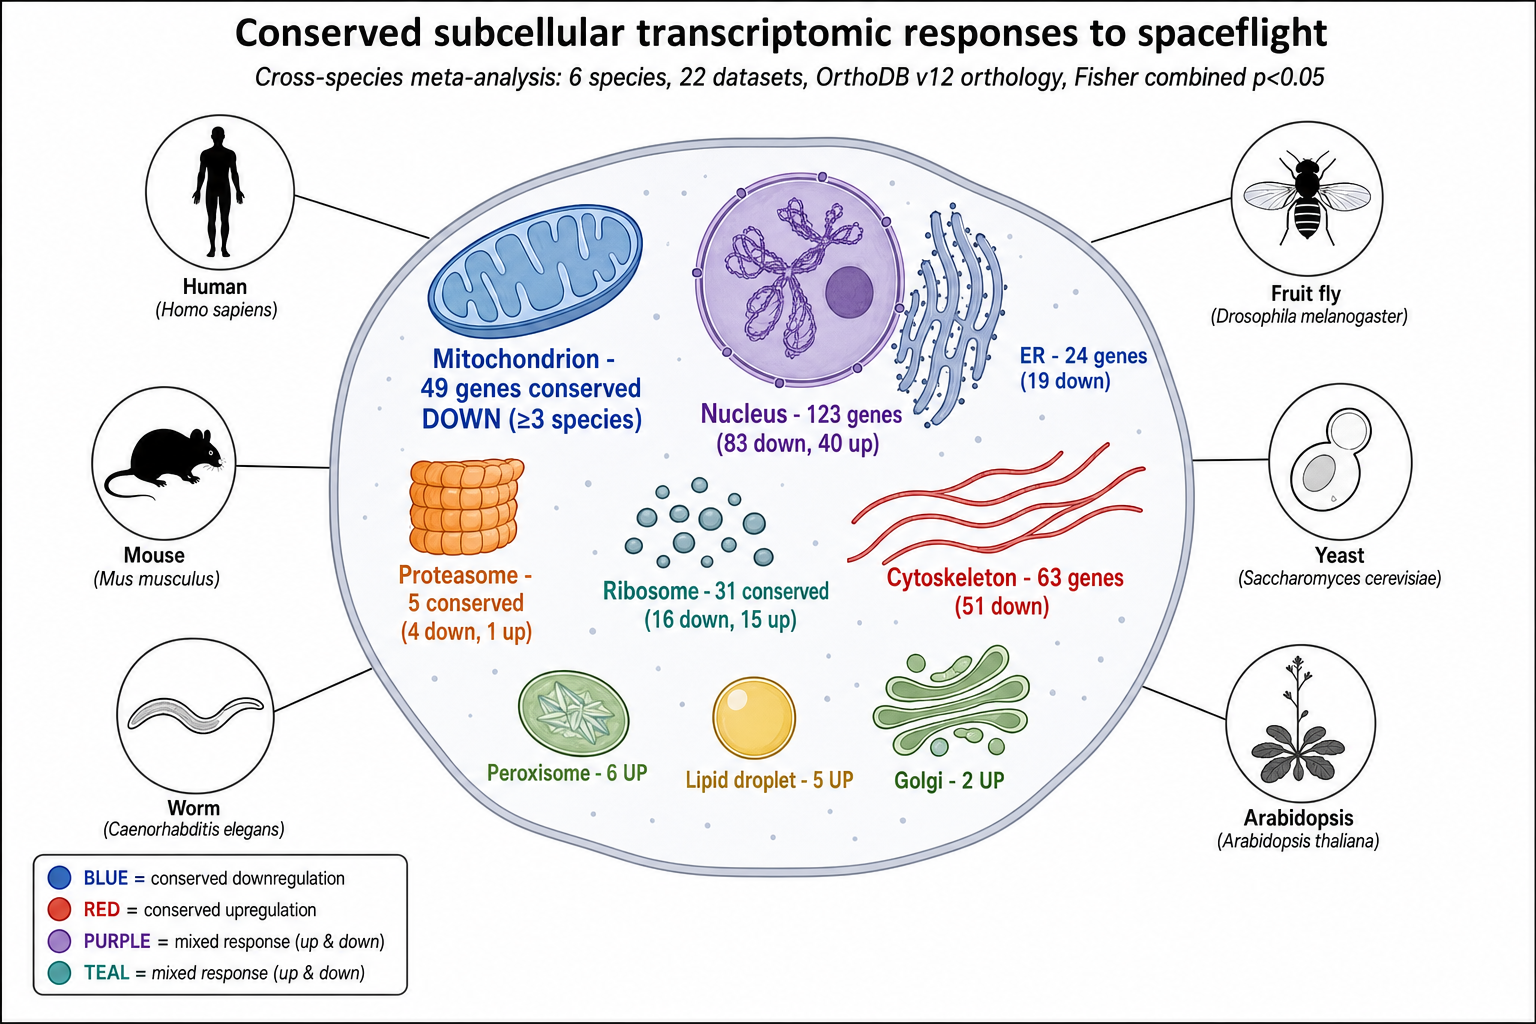
\includegraphics[width=0.9\textwidth]{fig5_conserved_organelle_schematic.png}
\caption{\textbf{Conserved subcellular transcriptomic responses to spaceflight.}
Schematic of a eukaryotic cell showing organelles with conserved transcriptional
responses across species. Blue indicates conserved downregulation, red indicates
conserved upregulation, and purple/teal indicate mixed responses. The
mitochondrion (49 genes, 100\% downregulated across \(\geq 3\) species) is the
most robustly conserved response. Numbers indicate conserved gene counts.}
\label{fig5}
\end{figure}

\subsection{Pathway-level visualization reveals cofactor-dependent divergence}

To examine the conserved mitochondrial suppression at pathway resolution, we
visualized four KEGG pathways (oxidative phosphorylation, proteasome, ribosome,
TCA cycle) using ggkegg, overlaying per-species mean log2FC values onto gene
nodes (Fig.~\ref{fig6}). This reveals that while the overall mitochondrial
suppression is conserved, individual complex components show species-specific
patterns.

In oxidative phosphorylation (hsa00190), \textit{Drosophila} shows the strongest
downregulation across Complex I, III, IV, and V components, while human and mouse
show more modest changes with some upregulation of specific subunits. \textit{C.\
elegans} and Arabidopsis show intermediate patterns. The TCA cycle (hsa00020)
shows more uniform downregulation across species, particularly for the isocitrate
dehydrogenase complex (IDH3A, IDH3B, IDH3G), consistent with the conservation
meta-analysis.

\begin{figure}[htbp]
\centering
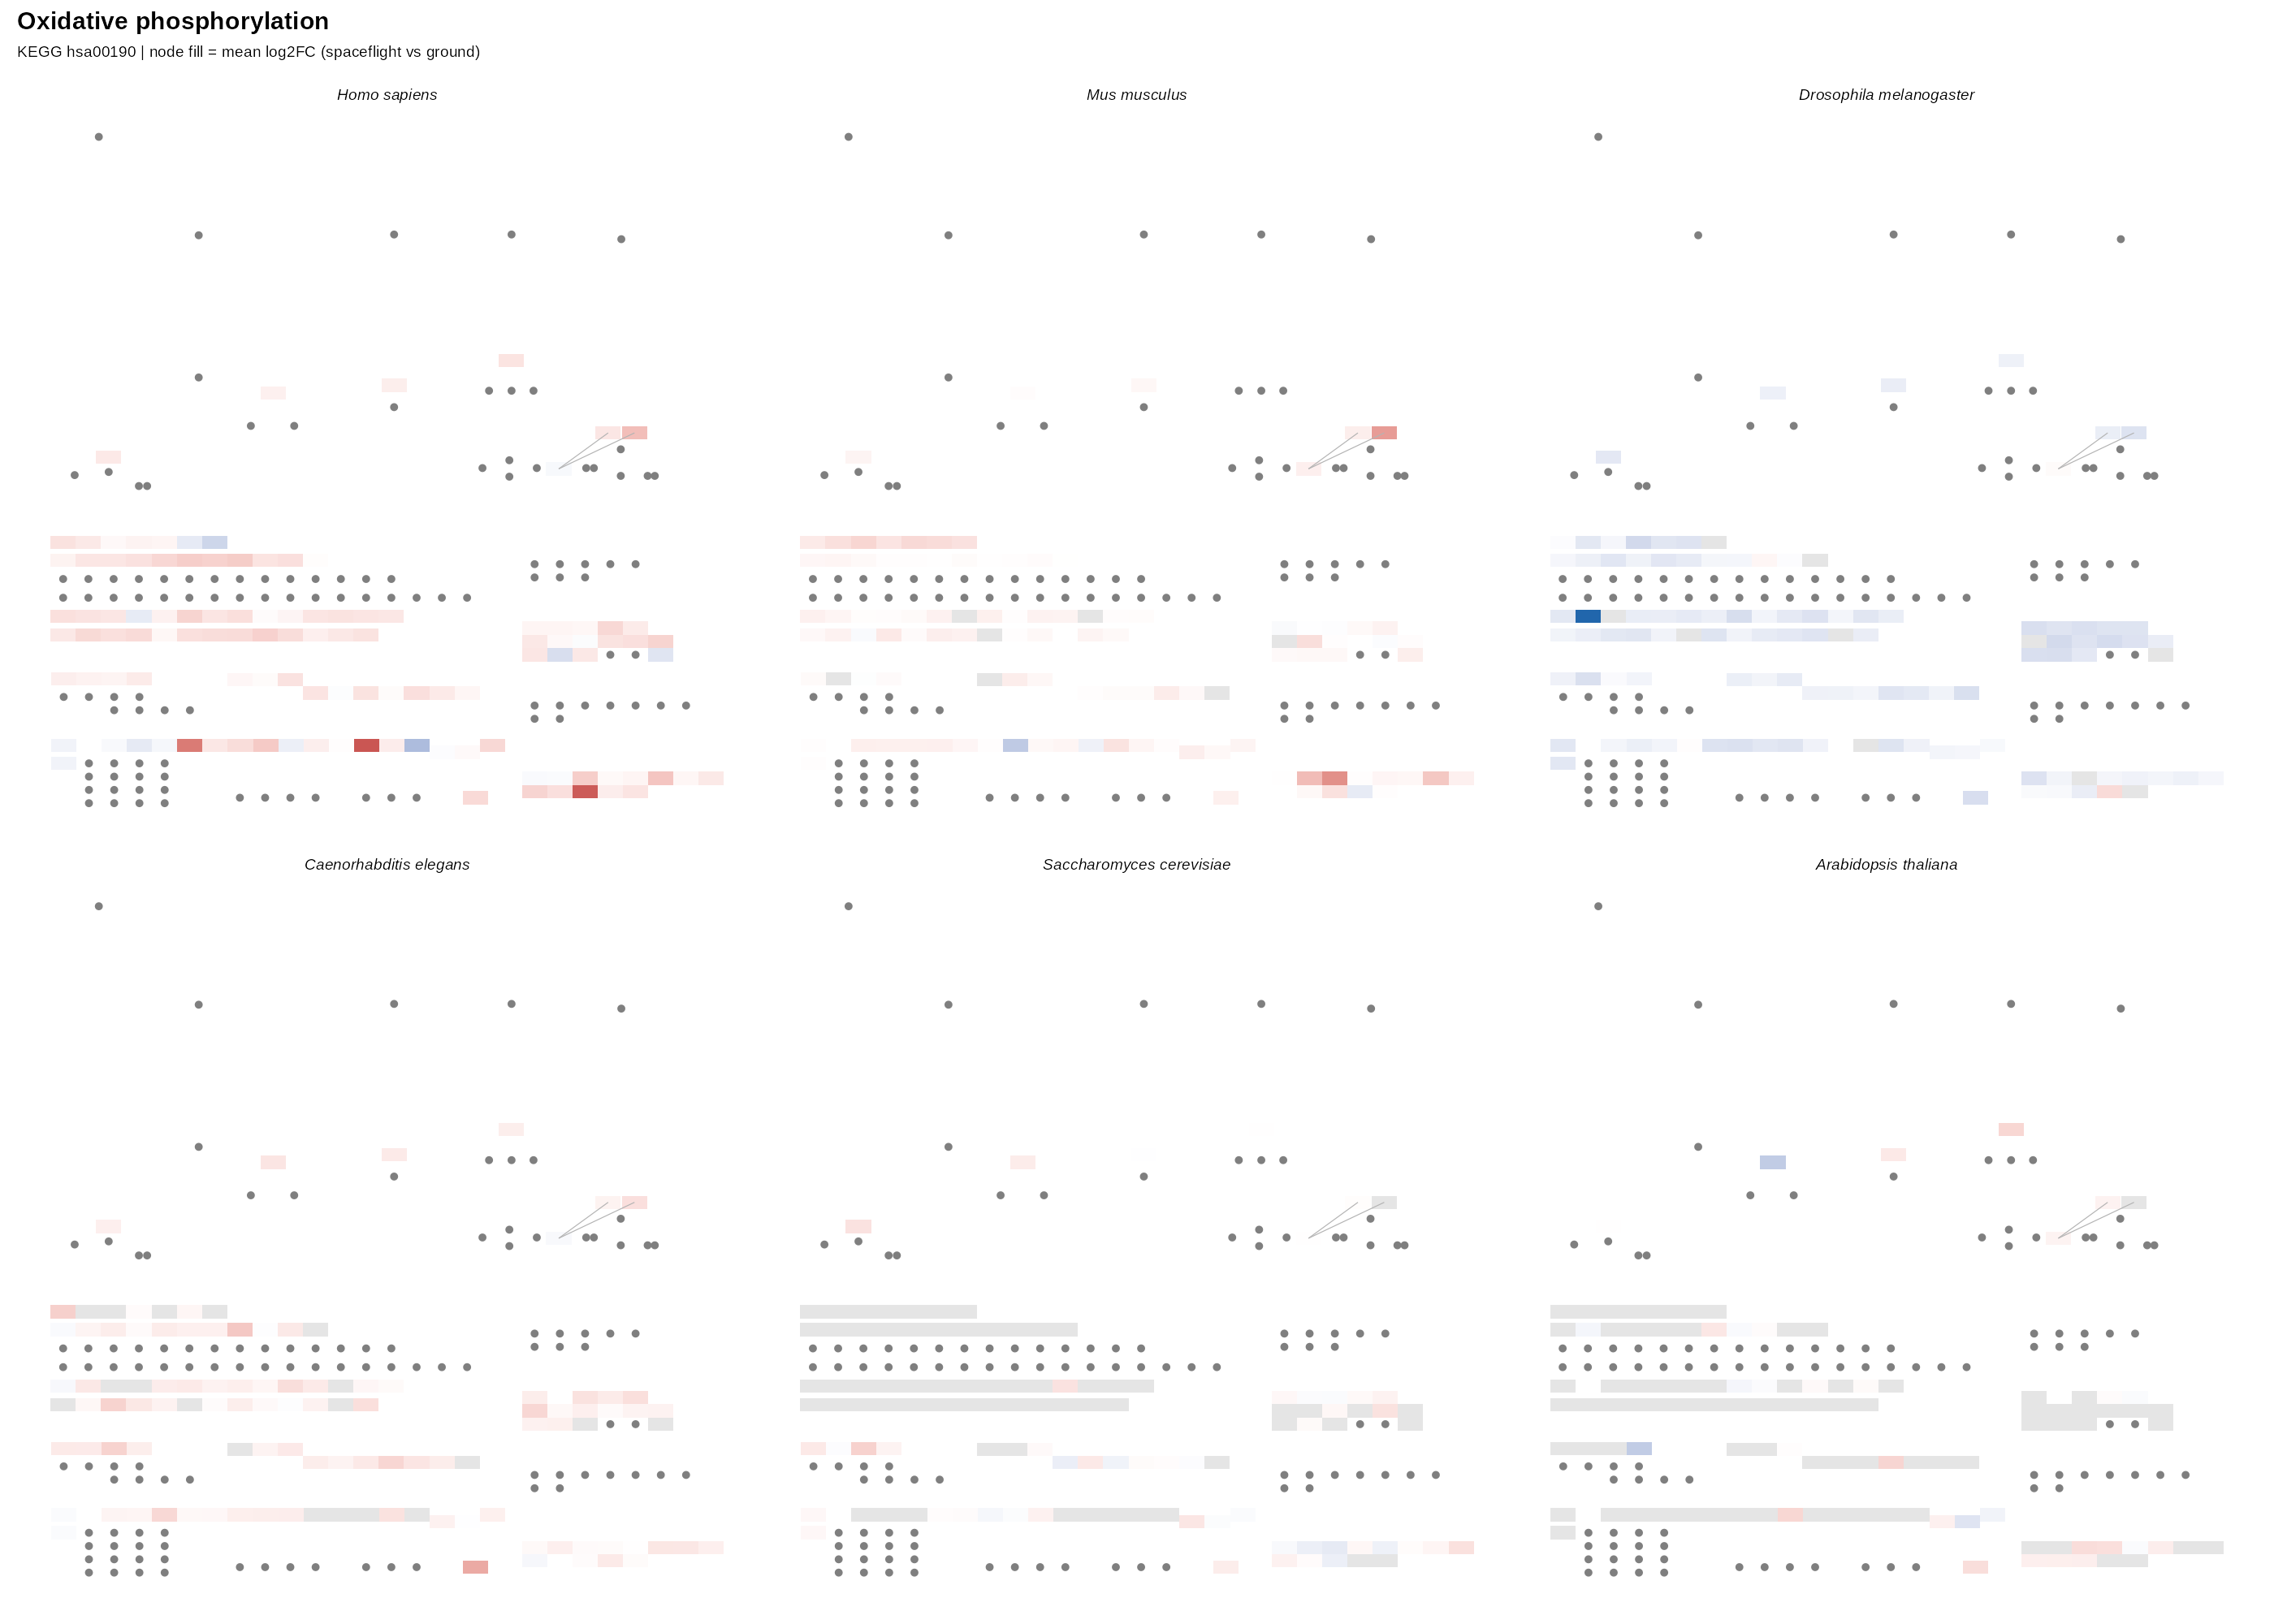
\includegraphics[width=\textwidth]{fig6_pathway_hsa00190.png}\\[1ex]
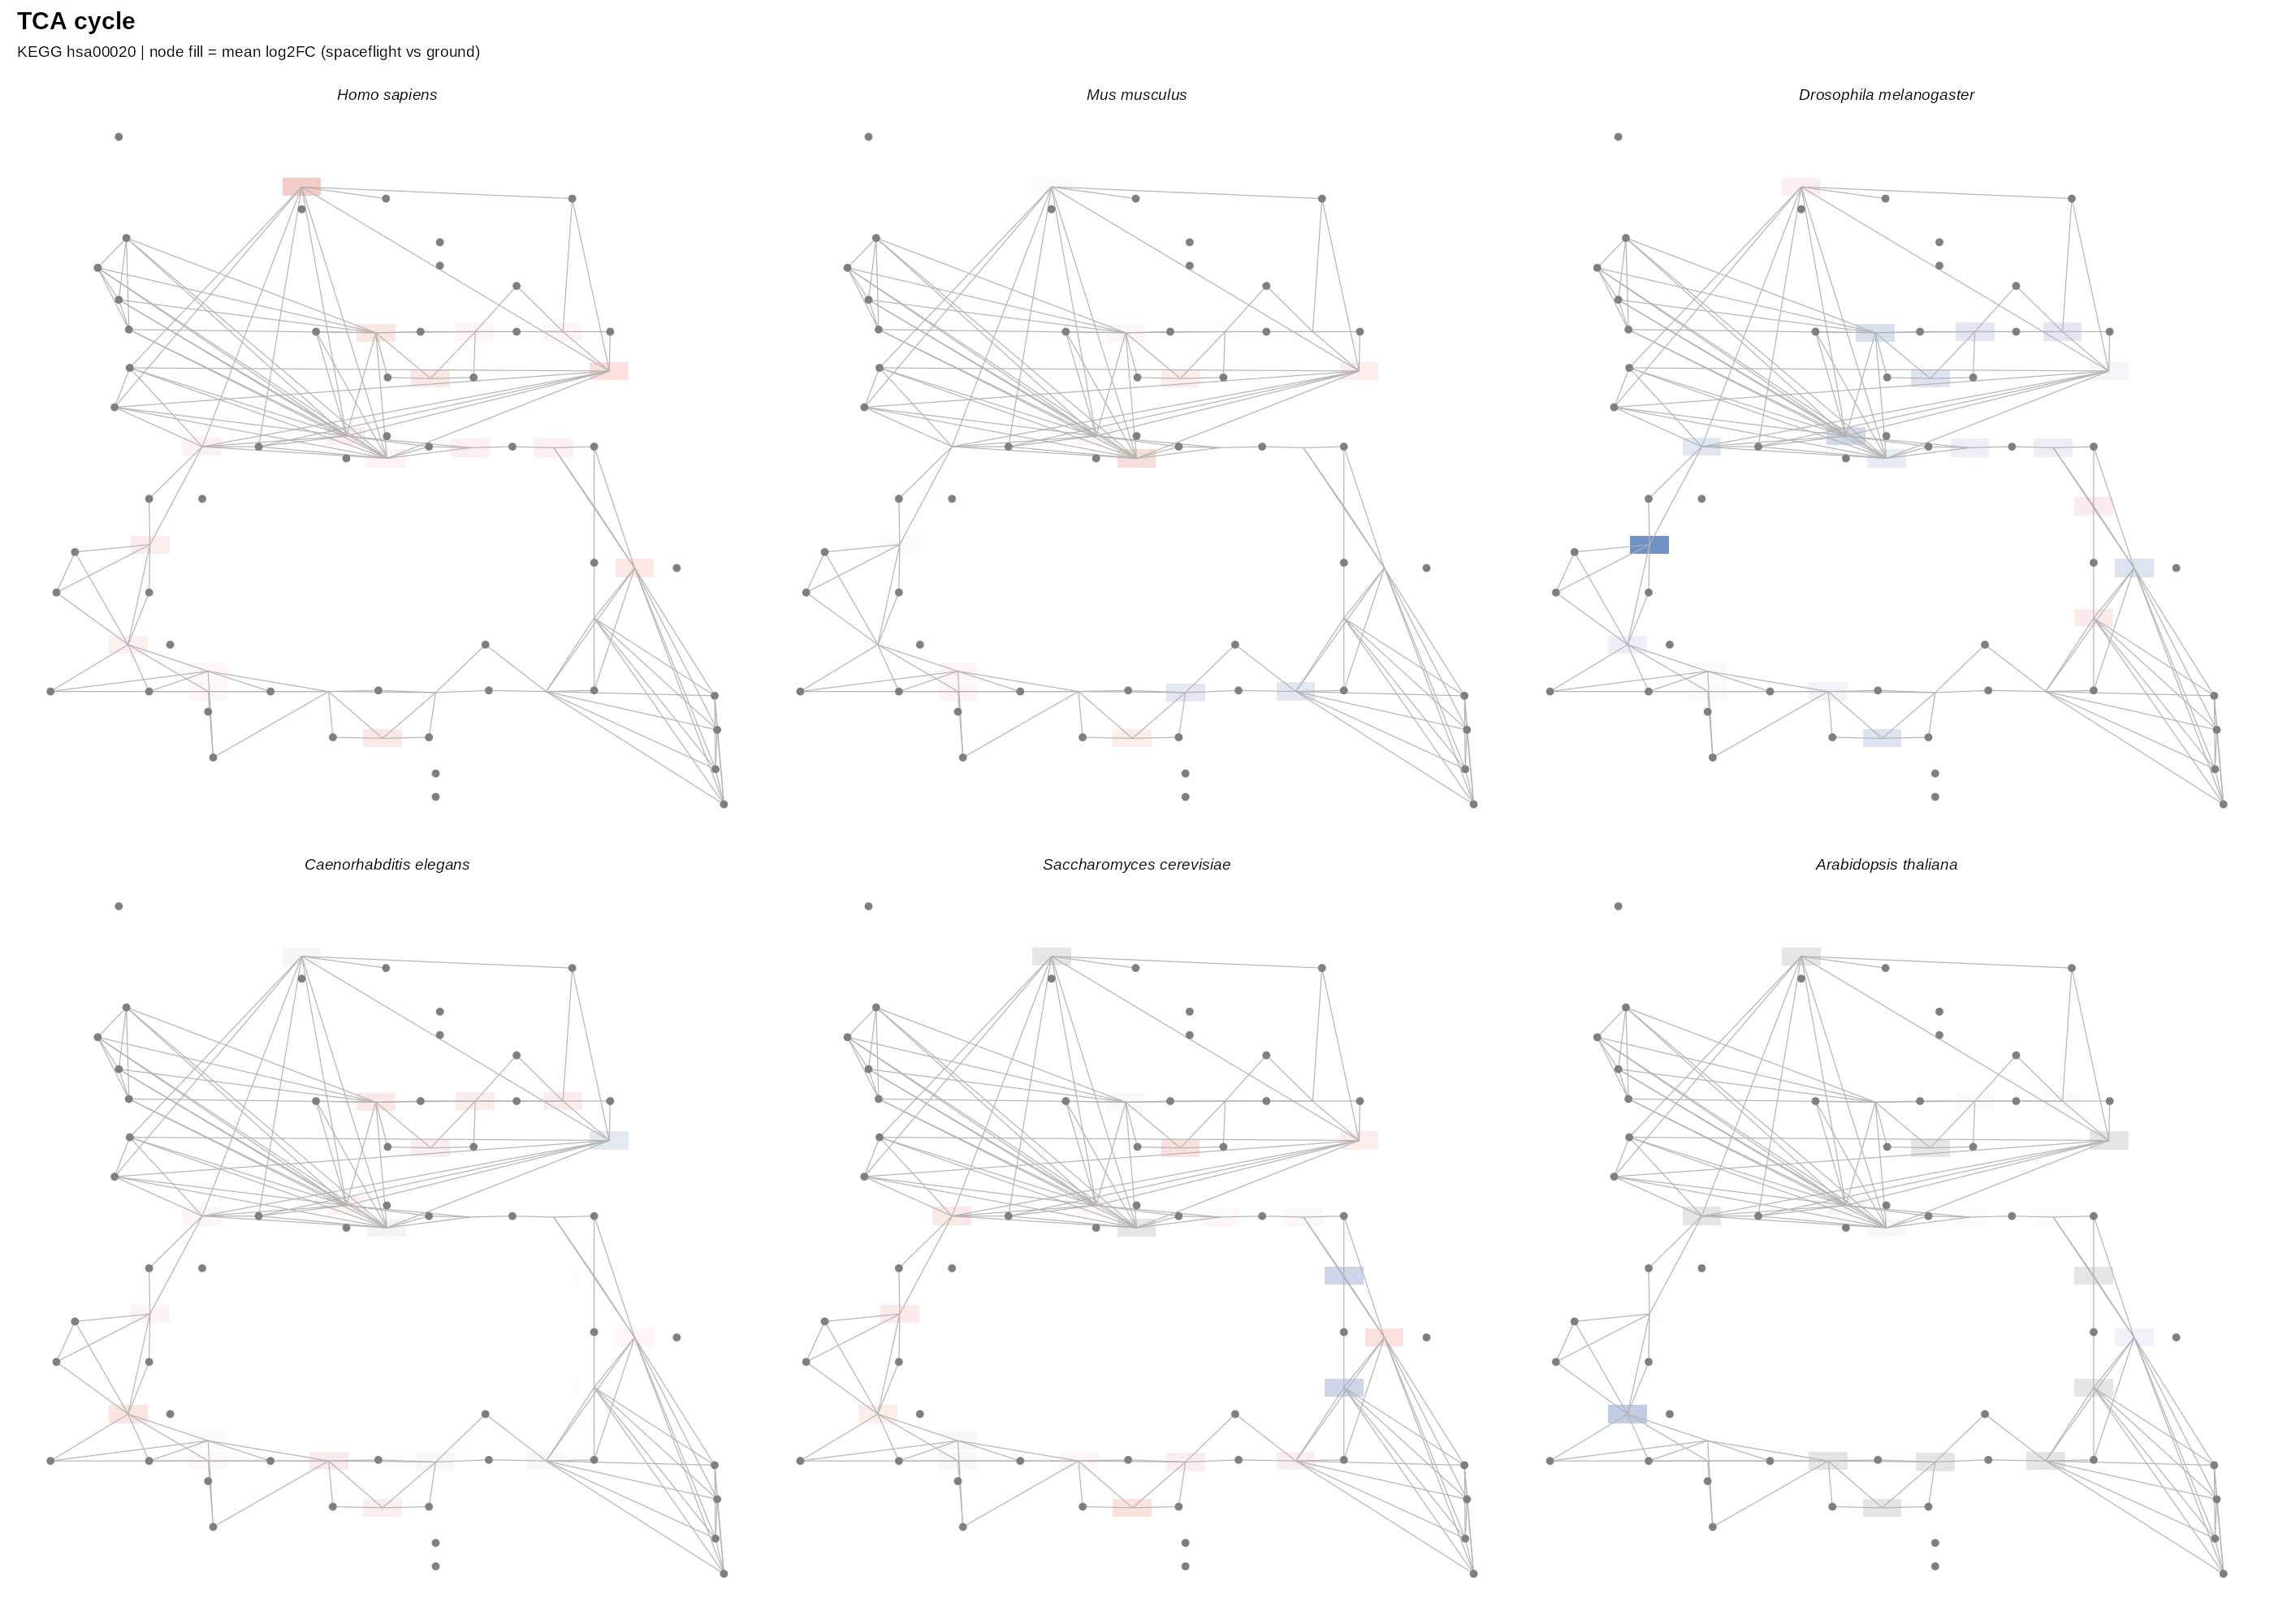
\includegraphics[width=\textwidth]{fig6_pathway_hsa00020.png}
\caption{\textbf{KEGG pathway diagrams with per-species log2FC overlay.} Top:
oxidative phosphorylation (hsa00190). Bottom: TCA cycle (hsa00020). Each panel
shows the KEGG pathway for one species, with gene nodes colored by mean log2FC
(blue = downregulated, red = upregulated, grey = no data). Diverging scale:
\(-2\) to \(+2\). Proteasome (hsa03050) and ribosome (hsa03010) are provided as
supplementary figures.}
\label{fig6}
\end{figure}

\subsection{Cofactor-dependent enzymes show species-divergent responses}

We mapped 14 enzyme cofactors to human genes via the KEGG
compound-reaction-enzyme-gene chain, yielding 498 unique genes across 12
cofactors (Fe-S cluster and Zn\textsuperscript{2+} returned no genes as KEGG
tracks these as prosthetic groups rather than reaction substrates). We then
examined the expression of cofactor-dependent enzymes across species and pathways
(Fig.~\ref{fig7}).

NAD\textsuperscript{+}/NADH-dependent enzymes, which dominate oxidative
phosphorylation, show species-divergent responses: downregulation in
\textit{Drosophila} (mean log2FC \(= -0.18\)) but upregulation in human (0.14) and
mouse (0.17). In contrast, CoA-dependent enzymes in the TCA cycle show more
variable but generally modest changes. TPP-dependent enzymes (pyruvate
dehydrogenase complex) show consistent downregulation in \textit{Drosophila} and
\textit{C.\ elegans}. Heme-dependent enzymes (cytochrome components) show
downregulation in \textit{Drosophila} and human but slight upregulation in yeast.
These cofactor-level patterns suggest that while the overall mitochondrial
suppression is conserved, the specific enzymatic routes affected vary by species,
potentially reflecting differences in metabolic strategy or redox buffering
capacity.

\begin{figure}[htbp]
\centering
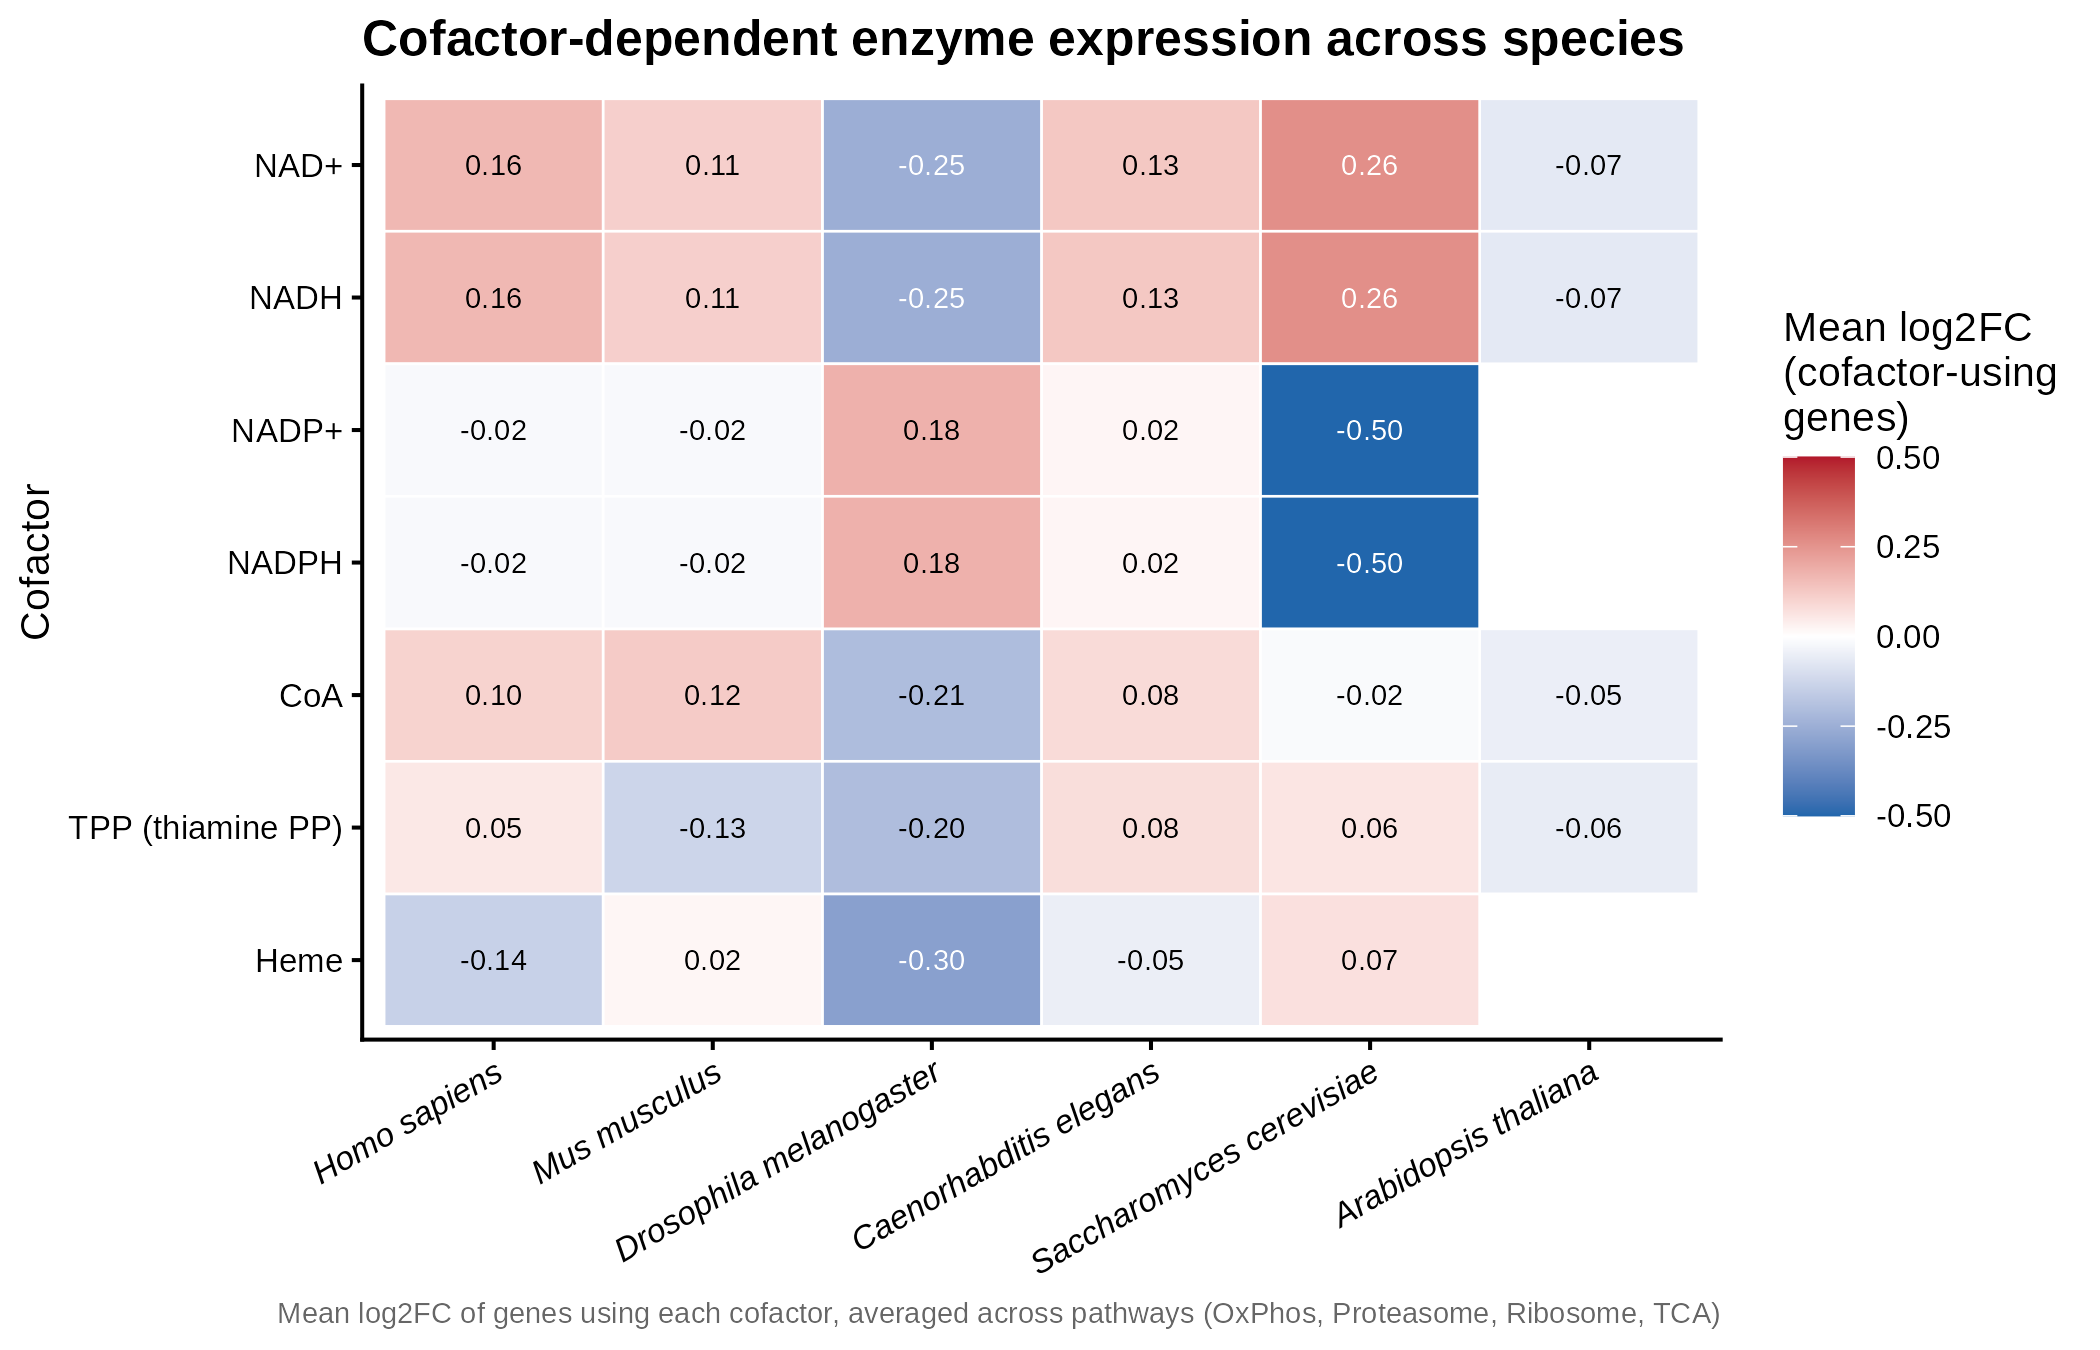
\includegraphics[width=0.9\textwidth]{fig7_cofactor_summary.png}
\caption{\textbf{Cofactor-dependent enzyme expression across species.} Heatmap
shows mean log2FC of genes using each cofactor, averaged across the four analyzed
pathways. Blue = downregulated, red = upregulated. NAD\textsuperscript{+}/NADH
enzymes show the most species-divergent pattern; CoA and TPP enzymes show more
conserved responses.}
\label{fig7}
\end{figure}

\section{Discussion}\label{sec:discussion}

Our cross-species meta-analysis reveals that mitochondrial gene suppression is the
most robustly conserved subcellular transcriptomic response to spaceflight, with
49 genes showing significant, direction-consistent downregulation across at least
three of six eukaryotic species spanning approximately one billion years of
evolution. This finding extends previous single-species observations of
mitochondrial dysregulation in spaceflight \cite{dasilva2021,mao2021,choi2021} to
a conserved, multi-kingdom response.

The specific genes identified paint a coherent biological picture: the conserved
suppression targets all five oxidative phosphorylation complexes (I--V) and key
TCA cycle enzymes, particularly the isocitrate dehydrogenase complex (IDH3A,
IDH3B, IDH3G). This suggests a coordinated reduction in oxidative capacity rather
than a stochastic effect. The conservation of this response from yeast to human
implies a fundamental cellular mechanism, potentially related to reduced energy
demand in microgravity, oxidative stress mitigation (reduced electron transport
reduces reactive oxygen species production), or a shift toward glycolytic
metabolism.

The contrast between conserved mitochondrial suppression and conserved peroxisome
and lipid droplet upregulation is intriguing. Peroxisomes are central to fatty
acid beta-oxidation and hydrogen peroxide metabolism, and their upregulation may
reflect compensatory responses to altered lipid metabolism or oxidative stress.
Lipid droplet accumulation has been observed in multiple spaceflight studies and
may relate to altered lipid handling in microgravity \cite{jonscher2016,zhang2022}.
The coordinated upregulation of Golgi apparatus genes suggests enhanced secretory
pathway activity, potentially related to extracellular matrix remodeling or stress
signaling.

Our cofactor analysis reveals an important nuance: while the overall mitochondrial
suppression is conserved, the specific enzymatic routes affected vary by species.
NAD\textsuperscript{+}/NADH-dependent enzymes show divergent responses (down in
fly, up in human and mouse), while CoA-dependent and TPP-dependent enzymes show
more conserved patterns. This suggests that species may employ different metabolic
strategies in response to spaceflight, with the conserved feature being a
reduction in specific mitochondrial functions rather than a uniform suppression of
all oxidative metabolism.

Several limitations should be noted. First, the datasets span different tissues,
durations, and experimental designs, introducing biological and technical
heterogeneity. We addressed this by using tissue as a covariate where possible and
applying tiered DEG thresholds, but residual heterogeneity remains. Second,
orthology mapping rates vary substantially across species, with Arabidopsis
particularly affected (3.2\% DEG mapping rate) due to the plant-specific gene
complement and reliance on OrthoDB rather than babelgene. Third, the yeast dataset
is a single microarray study with only 31 DEGs, limiting statistical power for
this species. Fourth, our conservation criterion requires significance in at least
three species, which may miss genuinely conserved responses that fall below
significance thresholds in individual datasets. Finally, transcriptomic changes do
not necessarily reflect protein-level or functional changes, and the relationship
between mRNA suppression and actual mitochondrial function in spaceflight requires
further validation.

Despite these limitations, the robustness of the mitochondrial suppression signal,
with Fisher combined \(p\)-values as low as \(10^{-68}\) and consistent direction
across diverse species, provides strong evidence for a conserved cellular
response. The identification of specific targets (IDH3B, CYC1, COX5B, ATP5F1A)
provides candidate biomarkers for monitoring mitochondrial responses to
spaceflight and potential targets for countermeasure development. Future work
should integrate proteomic and metabolomic data to validate the functional
consequences of these transcriptomic changes and explore whether pharmacological
mitigation of mitochondrial suppression is feasible and beneficial.

\section{Methods}\label{sec:methods}

\subsection{Data acquisition}
We queried the NASA OSDR Biological Data API
(\texttt{visualization.osdr.nasa.gov/biodata/api/v2/query/}) to enumerate RNA-seq
and microarray datasets with spaceflight versus ground control contrasts for six
species. The final selection comprised 22 datasets: OSD-37, 47, 48, 62, 96, 104,
105, 112, 113, 120, 207, 217, 242, 258, 323, 347, 35, 379, 421, 684, 863.
Processed data (DE tables, count matrices, sample tables) were downloaded via the
OSDR geode-py web service. Tissue metadata was extracted from the
\texttt{study.characteristics.material type} field.

\subsection{Differential expression analysis}
For 19 datasets, we used GeneLab RCP pre-computed DE tables (DESeq2
\cite{love2014} for RNA-seq, limma \cite{ritchie2015} for microarray). For OSD-96
(\textit{Drosophila} RSEM counts), we ran DESeq2 with design \(\sim\) tissue +
condition. For OSD-35 (\textit{C.\ elegans} microarray, no replicates), we ran
limma with nominal thresholds. We applied tiered DEG thresholds: standard
(\(p_{\mathrm{adj}} < 0.05\), \(|\text{log2FC}| > 1\)) for 19 datasets, relaxed
(\(p_{\mathrm{adj}} < 0.10\), \(|\text{log2FC}| > 0.5\)) for two datasets, and
nominal (\(p < 0.05\), \(|\text{log2FC}| > 0.5\)) for one dataset. Direction was
normalized so positive log2FC = upregulated in spaceflight.

\subsection{Orthology mapping}
We built a human-anchored orthology matrix using OrthoDB v12 \cite{kriventseva2023}
(\texttt{data.orthodb.org/v12/}) as the primary resource, supplemented by
babelgene \cite{gilbert2022} for human-to-mouse, fly, worm, and yeast mappings.
Arabidopsis TAIR IDs were mapped to human orthologs via OrthoDB Eukaryota-level
ortholog groups. The unified matrix comprises 18{,}030 human genes with at least
one non-human ortholog.

\subsection{Subcellular location enrichment}
We ran clusterProfiler \cite{yu2012} \texttt{enrichGO} (ontology = CC, \(p <
0.05\), Benjamini-Hochberg) per species for up- and down-regulated DEGs
separately, using species-specific \texttt{org.db} packages. Enriched terms were
manually classified into 16 organelle categories.

\subsection{Cross-species conservation meta-analysis}
For each organelle category, we applied Fisher's combined probability test
\cite{fisher1925} to per-species \(p\)-values for each orthologous gene, then
adjusted across all 1{,}210 tests using Benjamini-Hochberg FDR
\cite{benjamini1995}. A gene was considered conserved if Fisher FDR \(< 0.05\),
significant in \(\geq 3\) species, and direction-consistent (\(\geq 80\%\) same
direction).

\subsection{Pathway visualization and cofactor mapping}
KEGG \cite{kanehisa2016} pathway-gene links were fetched via the KEGG REST API
(\texttt{rest.kegg.jp}) for hsa00190, hsa03050, hsa03010, hsa00020. Cofactor-gene
mappings were built via the compound-reaction-enzyme-gene chain. Pathway diagrams
were rendered using ggkegg \cite{sato2023} with per-species log2FC overlays
(diverging blue-white-red scale, limits \(-2\) to \(+2\)); palettes use viridis
\cite{garnier2023}.

\subsection{AI use disclosure}
Data analysis scripting, figure generation, and manuscript drafting were assisted
by Biomni (Phylo). All statistical analyses, data interpretation, and scientific
conclusions were conducted and verified by the author. This AI assistance is
disclosed in accordance with npj Microgravity editorial policy.

\backmatter

\bmhead{Data availability}
All raw and processed data are available from the NASA Open Science Data
Repository (\texttt{osdr.nasa.gov}) using the OSD identifiers listed in Methods.
The complete analysis code, orthology matrices, supplementary tables, and figures
are deposited in a Zenodo repository (DOI to be assigned upon submission). OrthoDB
v12 data are available at \texttt{data.orthodb.org/v12/}. KEGG pathway data are
available at \texttt{kegg.jp}.

\bmhead{Code availability}
All analysis scripts (R) are available in the project repository under the
\texttt{scripts/} directory. The analysis used R 4.3 with DESeq2, limma,
clusterProfiler, ggkegg, babelgene, and OrthoDB v12 bulk files. Full software
requirements are listed in the repository README.

\bmhead{Acknowledgements}
We thank the NASA GeneLab consortium and the Open Science Data Repository for
providing open access to spaceflight omics data. This analysis was assisted by
Biomni (Phylo).

%% Supplementary Tables S1--S15 accompany this manuscript (see the repository
%% zenodo_repo/supplementary_tables/ folder).

\bibliography{references}

\end{document}
